\documentclass[11pt]{article}

\usepackage{geometry}
\geometry{margin=1in}
\usepackage[hyphens]{url}

\usepackage{mathtools}
%\usepackage{algpseudocode}
\usepackage{listings}
\usepackage{tikz}
\usepackage[nomessages]{fp}
\usepackage{adjustbox}
\usepackage{outlines}
%\usepackage{times}
\usepackage{graphicx,color}
\usepackage{array,float}
\usepackage{url}
%\usepackage[usenames,dvipsnames]{xcolor}
\usepackage{amstext,amssymb,amsmath}
\usepackage{hyphenat}
\usepackage{amsthm}
\usepackage{verbatim}
\usepackage{bm}
\usepackage{paralist}
\usepackage{ulem}\normalem
\usepackage[numbers]{natbib}
\usepackage{todonotes}
\usepackage{paralist}
\usepackage{wrapfig}
\usepackage{hyperref}
\usepackage[noend]{algorithmic}
\usepackage{algorithm}
\usepackage{commath}
\usepackage{needspace}
\usepackage{mathrsfs}

\newcommand{\rb}[1]{\textcolor{blue}{RB:#1}}
\newcommand{\al}[1]{\textcolor{blue}{AL:#1}}
\newcommand{\cz}[1]{\textcolor{blue}{CZ:#1}}


\newtheorem{lem}{Lemma}[section]
\newtheorem{thm}[lem]{Theorem}
\newtheorem{cor}[lem]{Corollary}
\newtheorem{problem}[lem]{Problem}
\newtheorem{defn}[lem]{Definition}
\newtheorem{fact}[lem]{Fact}
\newtheorem{remark}{Remark}
\newtheorem{example}{Example}
\newtheorem{assumption}[lem]{Assumption}
\newtheorem{claim}[lem]{Claim}
\newcommand{\ip}[2]{\left\langle #1,#2 \right\rangle}

\usepackage{dsfont}

\newcommand{\err}{\mathrm{err}}
\newcommand{\emperr}{\widehat{\err}}
\newcommand{\pr}[2]{\underset{#1}{\mathbb{P}}\left[ #2 \right]}
\newcommand{\ex}[2]{\underset{#1}{\mathbb{E}}\left[ #2 \right]}

\newcommand{\R}{\mathbb{R}}
\newcommand{\N}{\mathbb{N}}
\newcommand{\B}{\mathrm{B}}

\newcommand{\deriv}[2]{\frac{d #1}{d #2}}
\newcommand{\pDeriv}[2]{\frac{\partial #1}{\partial #2}}
\newcommand{\pDerivTwo}[3]{\frac{\partial^2 #1}{\partial #2 \partial #3}}

\newcommand{\cond}{\,|\,}

\newcommand{\quickFig}[2]{ %
  \begin{figure}[H] %
  \centering %
  \includegraphics[width=#1 \linewidth,natwidth=600]{#2} %
  \end{figure} %
}

\newcommand{\nth}{^{\mathrm{th}}}

\DeclareMathOperator*{\argmax}{arg\,max}
\DeclareMathOperator*{\argmin}{arg\,min}
\DeclareMathOperator*{\argsup}{arg\,sup}
\DeclareMathOperator*{\arginf}{arg\,inf}

\newcommand{\domain}{\mathop{\mathrm{domain}}}

\newcommand{\VC}{\mathop{\mathrm{VC}}}
\newcommand{\var}{\mathop{\mathrm{var}}}
\newcommand{\cov}{\mathop{\mathrm{cov}}}
\newcommand{\sign}{\mathop{\mathrm{sign}}}
\newcommand{\eps}{\varepsilon}


\newcommand{\bx}{\mathbf{x}}
\newcommand{\by}{\mathbf{y}}
\newcommand{\bz}{\mathbf{z}}
\newcommand{\bw}{\mathbf{w}}
\newcommand{\bu}{\mathbf{u}}
\newcommand{\bv}{\mathbf{v}}
\newcommand{\bp}{\mathbf{p}}
\newcommand{\cC}{\mathcal{C}}
\newcommand{\cH}{\mathcal{H}}
\newcommand{\cG}{\mathcal{G}}
\newcommand{\cF}{\mathcal{F}}
\newcommand{\cA}{\mathcal{A}}
\newcommand{\cX}{\mathcal{X}}
\newcommand{\zeroB}{\ensuremath{\mathbf{0}}}

\newcommand{\bigO}[1]{O\left(#1\right)}
\newcommand{\indi}[1]{\mathbf{1}\left(#1\right)}

\newcommand{\midvert}{\mathrel{}\middle\vert\mathrel{}}

\newcommand{\expect}[1]{\mathbb{E} \left[ #1 \right]}
\newcommand{\expectCond}[2]{\mathbb{E}%
    \left[ #1 \midvert #2 \right]}
\newcommand{\expectOver}[2]{\mathbb{E}_{\substack{#1}}\left[ #2 \right]}
\newcommand{\expectOverCond}[3]{\mathbb{E}_{\substack{#1}}%
    \left[ #2 \midvert #3 \right]}

\newcommand{\prob}[1]{\mathbb{P} \left( #1 \right)}
\newcommand{\probCond}[2]{\mathbb{P}%
    \left( #1 \midvert #2 \right)}
\newcommand{\probOver}[2]{\mathbb{P}_{\substack{#1}}\left( #2 \right)}
\newcommand{\probOverCond}[3]{\mathbb{P}_{\substack{#1}}%
    \left( #2 \midvert #3 \right)}

\lstset{basicstyle=\ttfamily}

\usepackage{etoolbox}

\newcommand{\surround}[2][r]%
  {\ifstrequal{#1}{round}%
    {\left( #2 \right)}%
    {\ifstrequal{#1}{square}%
      {\left[ #2 \right]}%
      {\ifstrequal{#1}{curly}%
        {\left\{ #2 \right\}}%
        {\ifstrequal{#1}{angle}%
          {\left\langle #2 \right\rangle}%
          {\ifstrequal{#1}{|}%
            {\left\lvert #2 \right\rvert}%
            {\ifstrequal{#1}{||}%
              {\left\lVert #2 \right\rVert}%
              {\ifstrequal{#1}{floor}%
                {\left\lfloor #2 \right\rfloor}%
                {\ifstrequal{#1}{ceil}%
                  {\left\lceil #2 \right\rceil}%
                  {\ifstrequal{#1}{.}%
                    {\left. #2 \right.}%
                    {\left( #2 \right)}%
                  }%
                }%
              }%
            }%
          }%
        }%
      }%
    }%
  }

\newcommand{\innerProduct}[2]{\surround[angle]{{#1}, {#2}}}


\newcommand{\KL}[2]{\textsc{KL}\left( {#1} , {#2} \right)}
%\newcommand{\KL}[2]{\textsc{KL}\left( {#1} \; \middle\Vert \; {#2} \right)}
\newcommand{\rKL}[2]{\textsc{ReversedKL}\left( {#1} , {#2} \right)}
\newcommand{\ELBO}{\mathrm{ELBO}}
\newcommand*{\placeholder}{\makebox[1ex]{$\cdot$}}
\newcommand{\sL}{\mathscr{L}}

\newcommand{\Discrete}{\mathrm{Discrete}}
\newcommand{\Gaussian}{\mathrm{Gaussian}}
\newcommand{\InverseGamma}{\mathrm{InverseGamma}}

\title{Notes on Coordinate Ascent Variational Inference}
\author{Andrew Leverentz}
\date{}

\begin{document}

\maketitle

\begin{sloppypar}
This document draws heavily upon ``Variational Inference: A Review for Statisticians'' (Blei et~al) and upon David Blei's lecture notes on Variational Inference.%
\footnote{Available at \url{https://www.cs.princeton.edu/courses/archive/fall11/cos597C/lectures/variational-inference-i.pdf}.}
However, I've modified some of the notation and expanded on some of the derivations in an attempt to make it more explicit and, I hope, a bit friendlier to newcomers like myself.
\end{sloppypar}

\section{Introduction}

Variational inference is a technique that can be used to approximate difficult-to-compute probability distributions.
Such distributions arise in Bayesian inference, where there is some vector $Z = (Z_1, \ldots, Z_m)$ of ``latent variables'' (or ``unobserved variables'') and some vector $X = (X_1, \ldots, X_n)$ of ``observed variables'' (often simply referred to as the observed data).
If we have a generative model for the joint distribution of $X$ and $Z$, we can express the posterior distribution (the probability of the latent variables given the observed variables) as
\begin{align}
p(Z = z \mid X = x) = \frac{p(Z=z, X=x)}{p(X=x)} = \frac{p(Z=z, X=x)}{\int p(Z = \tilde{z}, X = x) \, d\tilde{z}}.
\end{align}
Often, the denominator is intractable because it either involves integrals that cannot be evaluated directly or contains sums with a prohibitively large number of terms.

When computing the posterior, we assume that we have an observed set of data $x = (x_1, \ldots, x_n)$ which is fixed throughout the analysis.
Thus, the function we wish to approximate is a univariate function which maps vectors $z$ to $p(Z = z \mid X = x)$.
For conciseness, we will express this function as $p(\placeholder \mid X = x)$.
In order to find an approximation to the posterior distribution $p(\placeholder \mid X = x)$, we will define a mathematically convenient family of functions, from which we then search for the function which most closely resembles our target distribution.

\section{Minimizing KL Divergence}

The notion of closeness that we will use for comparing probability distributions is \emph{reversed Kullback-Leibler divergence}.
Given two functions $a$ and $b$ which define probability distributions over some set $S$ (often $\mathbb R^d$ for some $d \geq 1$), the Kullback-Leibler divergence is defined as
\begin{align}
\KL{a}{b}
&= \int_S a(z) \log \left( \frac{a(z)}{b(z)} \right) \, dz.
\end{align}
Sometimes, this is written more concisely as
\begin{align}
\KL{a}{b}
&= \expectOver{Z \sim a}{ \log \left( \frac{a(z)}{b(z)} \right) }.
\end{align}
If $S$ is a discrete set, then the integrals are replaced by sums.
Reversed KL divergence is nearly identical, but with the arguments swapped:
\[ \rKL{a}{b} = \KL{b}{a}. \]

For convenience, we assume that $p(\placeholder \mid X = x)$ can be reasonably well approximated by one or more members from a limited set of functions $Q$, which we define below.

For each latent variable $Z_k$, we choose a parameterized family of distributions, such as Gaussians or beta distributions.%
\footnote{Later, we'll see that it is often convenient to choose distributions which belong to the \emph{exponential family}, which is actually a set of sets of distributions.}
Let $q_k(z_k; \nu_k)$ denote the distribution we have selected corresponding to the $k\nth$ latent variable, parameterized by a vector $\nu_k$.
We refer to the components of $\nu_k$ as the \emph{variational parameters} corresponding to the latent variable $Z_k$.
Note that we can associate different latent variables with different parameterized families, and their underlying variational parameters can have different dimensions.

For example, we might choose $q_1$ to be a normal distribution, which requires two parameters ($\nu_{1,1} =$ the mean and $\nu_{1,2} =$ the standard deviation), while $q_2$ might be a Bernoulli distribution, which requires just one parameter ($\nu_{2,1} =$ the probability that the outcome equals 1).
In this case, we would write
\begin{align}
q_1(z_1; \nu_1) &= \frac{1}{\nu_{1,2} \sqrt{2 \pi}} \exp\left( -\frac{(z_1 - \nu_{1,1})^2}{2 (\nu_{1,2})^2} \right), \\
q_2(z_2; \nu_2) &=
    \begin{cases}
    1-\nu_{2,1}, & z_2 = 0, \\
    \nu_{2,1},   & z_2 = 1.
    \end{cases}
\end{align}
In this case, $\nu_{1,1}$ can be any real number, $\nu_{1,2}$ can be any positive real number, and $\nu_{2,1}$ can be any number in the interval $[0,1]$.

Once we select a parameterized family of distributions for each latent variable, we define $Q$ to be the set of functions of the form
\begin{align}
q(z; \nu_1, \ldots, \nu_m) = \prod_{j=1}^m q_j(z_j; \nu_j).
\end{align}
By restricting ourselves to functions that can be written as a product of $m$ functions $q_1(z_1; \nu_1)$ through $q_m(z_m; \nu_m)$, we are using what is known as the ``mean field'' approximation.
In order to make our notation less cumbersome, we will occasionally omit the variational parameters $\nu_j$.
In those cases, $q(z)$ should be interpreted to mean $q(z; \nu_1, \ldots, \nu_m)$, and $q_j(z_j)$ should be interpreted to mean $q_j(z_j; \nu_j)$.

Finally, we can formulate our approximation problem as the following:
given a target distribution $p(\placeholder \mid X=x)$ and a variational family of functions $Q$, find the function $q \in Q$ which minimizes the reversed KL divergence between $p(\placeholder \mid X = x)$ and $q$.
In mathematical notation, we wish to find
\begin{align}
q^*
&= \argmin_{q \in Q} \rKL{p(\placeholder \mid X = x)}{q} \\
&= \argmin_{q \in Q} \KL{q}{p(\placeholder \mid X = x)} \\
&= \argmin_{q \in Q} \int q(z) \log \left( \frac{q(z)}{p(Z = z \mid X = x)} \right) \, dz.
\end{align}
We can use the fact that $q$ is a probability distribution (since products of probability distributions are also probability distributions) to express this more concisely:
\begin{align}
\Aboxed{
q^*
&= \argmin_{q \in Q} \expectOver{Z \sim q}{ \log \left( \frac{q(Z)}{p(Z \mid X = x)} \right) }.
}
\label{eq:qstarUnsimplified}
\end{align}

There are two useful ways to rewrite equation \eqref{eq:qstarUnsimplified}.
First, we can write $q^*$ without any conditional probabilities:
\begin{align}
q^*
&= \argmin_{q \in Q} \expectOver{Z \sim q}{ \log \left( \frac{q(Z) \, p(X = x)}{p(Z, X = x)} \right) } \\
&= \argmin_{q \in Q} \expectOver{Z \sim q}{ \log q(Z) + \log p(X = x) - \log p(Z, X = x) } \\
\label{eq:takePXout}
&= \argmin_{q \in Q} \left(
    \log p(X = x) + \expectOver{Z \sim q}{ \log q(Z) } - \expectOver{Z \sim q}{ \log p(Z, X = x) }
    \right) \\
\label{eq:removePX}
&= \argmin_{q \in Q} \left(
    \expectOver{Z \sim q}{ \log q(Z) } - \expectOver{Z \sim q}{ \log p(Z, X = x) }
    \right) \\
\label{eq:switchToMax}
&= \argmax_{q \in Q} \left(
    \expectOver{Z \sim q}{ \log p(Z, X = x) } - \expectOver{Z \sim q}{ \log q(Z) }
\right).
\end{align}
In \eqref{eq:takePXout}, we take $\log p(X = x)$ out of the expectation because it does not depend on $Z$.
Then, in \eqref{eq:removePX}, we drop that term completely, because it does not depend on $q$ at all, and therefore it does not affect the optimal value.
In \eqref{eq:switchToMax}, we see that minimizing the reversed KL divergence is equivalent to maximizing the following quantity:
\begin{align}
\label{eq:ELBO}
\ELBO
&= \expectOver{Z \sim q}{ \log p(Z, X = x) } - \expectOver{Z \sim q}{ \log q(Z) }.
\end{align}
This quantity is known as the ``evidence lower bound'' (abbreviated ELBO) because it lower-bounds the logarithm of the probability of the observed data, $\log p(X = x)$.
To see why, note that
\begin{align}
\log p(X = x)
&= \log \int p(Z = z, X = x) \, dz \\
&= \log \int p(Z = z, X = x) \frac{q(z)}{q(z)} \, dz \\
&= \log \expectOver{Z \sim q}{ \frac{p(Z, X=x)}{q(Z)} } \\
\label{eq:elboFromJensen}
&\geq \expectOver{Z \sim q}{ \log \frac{p(Z, X=x)}{q(Z)} } \\
&= \ELBO.
\end{align}
The inequality in \eqref{eq:elboFromJensen} comes from Jensen's inequality, since $\log(\placeholder)$ is a concave function.
When implementing variational inference, it can be useful to track the ELBO over the course of the optimization to assess convergence.
The ELBO is easier to compute than the reversed KL divergence, because (1) we know the joint probability of $Z$ and $X$, and (2) since $q$ is assumed to be in a nicely factorable form, computing $q(Z)$ is tractable.

Returning to \eqref{eq:qstarUnsimplified}, we can rewrite our expression for $q^*$ by noting that $q(Z) = \prod_{j=1}^m q_j(Z_j)$:
\begin{align}
q^*
&= \argmin_{q \in Q} \left(
    \left[ \sum_{j=1}^m \expectOver{Z_j \sim q_j}{\log q_j(Z_j; \nu_j)} \right]
    -
    \expectOver{Z \sim q}{\log p(Z \mid X = x)}
\right).
\end{align}

Let $\sL$ denote the quantity to be optimized; that is,
\begin{align}
\label{eq:beforeRemovingConstWrtK}
\sL
&=
\left[ \sum_{j=1}^m \expectOver{Z_j \sim q_j}{\log q_j(Z_j; \nu_j)} \right]
    -
    \expectOver{Z \sim q}{\log p(Z \mid X = x)}.
\end{align}

\section{Coordinate Ascent}

At this point, a common approach is to search for the optimal value $q^*$ using coordinate ascent.
That is, we first optimize the parameters $\nu_1$ corresponding to $q_1$, holding all other variational parameters fixed.
Then, we optimize the parameters $\nu_2$ corresponding to $q_2$, holding all others fixed, and so on.
We repeatedly optimize $\nu_1, \ldots, \nu_m$ until we reach convergence (which we can roughly assess by monitoring the ELBO).

Let $Z_{-k}$ denote all random variables in the vector $Z$ except for $Z_k$.
That is, \begin{equation} Z_{-k} = (Z_1, \ldots, Z_{k-1}, Z_{k+1}, \ldots, Z_m). \end{equation}
Similarly, let $\mathbb E_{Z_{-k} \sim q_{-k}}$ denote an expectation where $Z_j \sim q_j$ for all $j \neq k$.
(Thus, if $z_k$ appears in such an expression, it is treated as a constant.)
Then, note that for each $k \in \{1, \ldots, m\}$, we can write
\begin{align}
\expectOver{Z \sim q}{\log p(Z \mid X = x)}
&= \expectOver{Z \sim q}{ \log \left( p(Z_{-k} \mid X = x) \, p(Z_k \mid Z_{-k}, X = x) \right) } \\
%&= \expectOver{Z \sim q}{ \log p(Z_{-k} \mid X = x) + \log p(Z_k \mid Z_{-k}, X = x) } \\
%
&= \begin{aligned}[t]
&\expectOver{Z_{-k} \sim q_{-k}}{ \log p(Z_{-k} \mid X = x) } \\
&+ \expectOver{Z \sim q}{ \log p(Z_k \mid Z_{-k}, X = x) }
\end{aligned} \\
%
&= \begin{aligned}[t]
&\expectOver{Z_{-k} \sim q_{-k}}{ \log p(Z_{-k} \mid X = x) } \\
&+ \expectOver{Z_k \sim q_k}{ \expectOver{Z_{-k} \sim q_{-k}}{ \log p(Z_k \mid Z_{-k}, X = x) } }.
\end{aligned}
\end{align}
In the last step, we have simply split an expectation over all of $Z$ into an expectation over all variables except $Z_k$, followed by an expectation over $Z_k$.

Next, we return to \eqref{eq:beforeRemovingConstWrtK} and rewrite $\sL$ as
\begin{align}
\sL
&= C_k
    + \expectOver{Z_k \sim q_k}{\log q_k(Z_k; \nu_k)}
    - \expectOver{Z_k \sim q_k}{ \expectOver{Z_{-k} \sim q_{-k}}{ \log p(Z_k \mid Z_{-k}, X = x) } },
\end{align}
where $C_k$ is the sum of all the terms that do not depend on $q_k$.
This is equivalent to
\begin{align}
\sL
&= \begin{aligned}[t]
    & C_k + \int
       q_k(z_k; \nu_k) \log q_k(z_k; \nu_k) \, dz_k \\
    & - \int q_k(z_k; \nu_k) \, \expectOver{Z_{-k} \sim q_{-k}}{ \log p(Z_k = z_k \mid Z_{-k}, X = x) } dz_k.
    \end{aligned}
\end{align}

Thus, for any $k \in \{1, \ldots, m\}$, we can express the quantity to be optimized as a functional%
\footnote{In this context, a functional is a function that takes as input a function ${\mathbb R \to \mathbb R}$ and returns a real value.  The ``type signature'' of a functional is ${(\mathbb R \to \mathbb R) \to \mathbb R}$.}
of $q_k$.
To find the value of $q_k$ that yields the minimal value of $\sL$ (while holding $q_j$ fixed for all $j \neq k$), we will compute the functional derivative of $\sL$ with respect to $q_k$.
Then, we will compute the value of $q_k$ that causes the functional derivative of $\sL$ to be zero.

The functional derivative $\delta\sL / \delta q_k$ is the functional which satisfies the following equation,%
    \footnote{Source: \url{https://en.wikipedia.org/wiki/Functional_derivative}.
    Note that $\sL$ has the type signature ${(\mathbb R \to \mathbb R) \to \mathbb R}$, whereas the functional derivative of $\sL$ with respect to $q_k$ has the type signature ${(\mathbb R \to \mathbb R) \to (\mathbb R \to \mathbb R)}$.
    In other words, the functional derivative is a function which takes two inputs, (1) a function ${\mathbb R \to \mathbb R}$ and (2) a real number, and outputs a real number.}
for any function $\phi : \mathbb R \to \mathbb R$:%
\begin{align}
\int \left( \frac{\delta \sL}{\delta q_k}[q_k](z_k) \right) \phi(z_k) \, dz_k
&=
\frac{d}{d\epsilon} \biggl[
    \sL[q_k + \epsilon \phi]
\biggr]_{\epsilon = 0}
\end{align}

We can compute the right-hand side and extract an expression for $\delta\sL / \delta q_k$, or we can take a shortcut by noting that the functional derivative of $\int f(q_k(z_k)) \, dz_k$ with respect to $q_k$ is simply $f'(q_k(z_k))$, for any $f$.
The result is that
\begin{align}
\frac{\delta \sL}{\delta q_k}[q_k](z_k)
&= 1 + \log q_k(z_k; \nu_k)
- \expectOver{Z_{-k} \sim q_{-k}}{ \log p(Z_k = z_k \mid Z_{-k}, X = x) }.
\end{align}

Setting this equal to zero and solving for $q_k$, we have
\begin{align}
\label{eq:generalCoordAscentCond}
\Aboxed{
q_k(z_k; \nu_k)
&= C_0 \exp \left( \expectOver{Z_{-k} \sim q_{-k}}{ \log p(Z_k = z_k \mid Z_{-k}, X = x) } \right),
}
\end{align}
where $C_0$ is a normalizing constant that does not depend on $z_k$.

We can also eliminate the conditional probability in this formula by noting that
\begin{align}
p(Z_k = z_k \mid Z_{-k}, X = x)
&= \frac{p(Z_k = z_k, Z_{-k}, X = x)}{p(Z_{-k}, X = x)}.
\end{align}
Since the denominator does not depend on $z_k$, we can instead write
\begin{align}
\label{eq:generalCoordAscentNoCond}
\Aboxed{
q_k(z_k; \nu_k)
&= C'_0 \exp \left( \expectOver{Z_{-k} \sim q_{-k}}{ \log p(Z_k = z_k, Z_{-k}, X = x) } \right),
}
\end{align}
where $C'_0$ is a new normalizing constant; in particular,
\begin{align}
C'_0 = C_0 \exp \left( -\expectOver{Z_{-k} \sim q_{-k}}{ \log p(Z_{-k}, X = x) }\right).
\end{align}

Therefore, each coordinate-ascent update step consists of computing either \eqref{eq:generalCoordAscentCond} or \eqref{eq:generalCoordAscentNoCond}, whichever happens to be more convenient for the given model.

\section{The Exponential Family}

At this point, we note that finding this optimal update becomes straightforward if we make careful choices regarding the structure of our model and the corresponding variational family $Q$.
In particular, suppose that we can construct our model so that the conditional probabilities are all in the exponential family (which we define below).
Suppose also that our model uses conjugate prior distributions where possible, so that the posterior distributions are all in the same family as the corresponding priors.
Furthermore, suppose that we select each $q_k$ to belong to the same parameterized family of distributions as the corresponding conditional of $Z_k$.
Under these assumptions, we will see that there is a simple formula for updating the variational parameters.

The \emph{exponential family} is a collection of parameterized sets of distributions whose probability densities can be written in the following form:
\begin{align}
p(X = x) = h(x) \exp\left[ \eta(\theta) \cdot T(x) - A(\eta(\theta)) \right].
\end{align}
A wide range of distributions, including Gaussian distribtions, categorical distributions, and many others, can be written in this form.%
\footnote{The Wikepedia article \url{https://en.wikipedia.org/wiki/Exponential_family} has a useful table of distributions in the exponential family, along with their natural parameters $\eta(\theta)$ and sufficient statistics $T(x)$.}
Here, $\eta$ is a vector-valued function that depends only on the parameters $\theta$ of the model.
The components of the vector $\eta(\theta)$ are called the \emph{natural parameters} of the distribution.
Often, the parameterization in terms of $\eta(\theta)$ is more mathematically convenient than the original parameterization (which is in terms of $\theta$).
However, the original parameterization is still occasionally useful, since the parameters $\theta$ typically have a more intuitive interpretation than the natural parameters $\eta(\theta)$.
In the special case where $\eta(\theta) = \theta$, the distribution is said to be in \emph{canonical form}.
Furthermore, $h$ and $T$ are functions that depend only on the random variable;
here, $h$ is scalar-valued, but $T$ may be vector-valued.
The components of $T(x)$ are known as the \emph{sufficient statistics} of the distribution.
Lastly, the function $A$ is a normalizing factor that causes the distribution to integrate to $1$.

If we assume that each conditional distribution in the model can be expressed as a member of the exponential family, and if we use conjugate-prior distributions wherever possible, then we have
\begin{align}
p(Z_k = z_k \mid Z_{-k} = z_{-k}, X = x) = h_k(z_k) \exp\left[ \eta_k(z_{-k}, x) \cdot T_k(z_k) - A_k(\eta_k(z_{-k}, x) \right].
\end{align}
Note that we have expressed the natural parameters of this distribution as a function of $z_{-k}$ and $x$.
Moreover, we have written $h_k$, $\eta_k$, $T_k$, and $A_k$ to emphasize that these functions can differ for distinct latent variabes $Z_k$.
We may occasionally write these functions without the subscript $k$, but we should keep in mind that there may be different functions for different latent variables.

In this context, we can write the update rule from \eqref{eq:generalCoordAscentCond} in a simpler form.
First, note that
\begin{align}
\expectOver{Z_{-k} \sim q_{-k}}{ \log p(z_k \mid Z_{-k}, X = x) }
&= \begin{aligned}[t]
    &\log h_k(z_k) \\
    &+ \expectOver{Z_{-k} \sim q_{-k}}{ \eta_k(Z_{-k}, x) } \cdot T_k(z_k) \\
    &- \expectOver{Z_{-k} \sim q_{-k}}{ A_k(\eta_k(Z_{-k}, x)) }.
    \end{aligned}
\end{align}
The final term is constant with respect to $z_k$, and so we can rewrite \eqref{eq:generalCoordAscentCond} as
\begin{align}
q_k(z_k; \nu_k)
&=
C''_0 \, h_k(z_k) \exp\left( \expectOver{Z_{-k} \sim q_{-k}}{\eta_k(Z_{-k}, x)} \cdot T_k(z_k) \right).
\end{align}
This shows that $q_k$ belongs to the same family as the distribution $p(Z_k = z_k \mid Z_{-k} = z_{-k}, X = x)$.
Thus, the optimal update for the parameters $\nu_k$ corresponding to $q_k$ can be extracted directly from the dot product in the previous equation:
\begin{align}
\label{eq:paramUpdate}
\Aboxed{
\nu_k
&=
\eta_k^{-1} \left(
    \expectOver{Z_{-k} \sim q_{-k}}{ \eta_k(Z_{-k}, x) }
\right).
}
\end{align}
Here, $\eta_k^{-1}$ is the inverse parameter mapping associated with $Z_k$, which maps the natural parameters back to our chosen parameterization.

Note that if we wish to use \eqref{eq:generalCoordAscentNoCond} instead of \eqref{eq:generalCoordAscentCond},
we simply replace $p(Z_k = z_k \mid Z_{-k} = z_{-k}, X = x)$ with $p(Z_k = z_k, Z_{-k} = z_{-k}, X = x)$ in the above analysis.

\section{Example: Mixture of Multivariate Gaussians}

Consider the following generative model for clustered data:
\begin{alignat}{2}
c_i &\sim \Discrete(r), &&\text{ for } i = 1, \ldots, n, \\
\mu_{k, \ell} &\sim \Gaussian(0, \alpha), &&\text{ for } k = 1, \ldots, K, \; \ell = 1, \ldots, d, \\
\lambda_{k, \ell} &\sim \InverseGamma(\beta_1, \beta_2), &&\text{ for } k = 1, \ldots, K, \; \ell = 1, \ldots, d, \\
x_i \mid c_i, \mu_{1:K,1:d}, \lambda_{1:K,1:d} &\sim \Gaussian(\mu_{c_i}, \Sigma_{c_i}), &&\text{ for } i = 1, \ldots, n.
\end{alignat}

Here, we define $\Sigma_k$ in terms of the random variables $\lambda_{k,\ell}$:
\begin{align}
\Sigma_k
= \begin{bmatrix}
    \lambda_{k, 1} & 0 & 0 & 0 \\
    0 & \lambda_{k, 2} & 0 & 0 \\
    0 & 0 & \ddots & 0 \\
    0 & 0 & 0 & \lambda_{k, d}
  \end{bmatrix}
\end{align}

In this model, $x_i$ represents the observed data, whereas $c_i$, $\mu_{k, \ell}$, and $\lambda_{k,\ell}$ are latent variables.
The values $r$, $\alpha$, $\beta_1$, and $\beta_2$ are fixed hyperparameters (in particular, $r$ is a $K$-dimensional vector which sums to $1$).

The intuition behind this model is as follows:
\begin{itemize}
    \item Each cluster $k \in \{1, \ldots, K\}$ is assigned a $d$-dimensional mean vector $\mu_k$.
    \item Each cluster $k \in \{1, \ldots, K\}$ is assigned a $d \times d$ diagonal covariance matrix $\Sigma_k$ corresponding to the $d$-dimensional vector $\lambda_k$.
    \item For each $i \in \{1, \ldots, n\}$, we select a cluster assignment $c_i \in \{1, \ldots, K\}$.
    \item Given all of the above information, each data point is sampled from a multivariate Gaussian with mean $\mu_{c_i}$ and covariance matrix $\Sigma_{c_i}$.
\end{itemize}

This yields the following probability densities:
\begin{align}
p(c_i) &= r_{c_i}, \\
p(\mu_{k, \ell}) &= (2\pi)^{-1/2} \, \alpha^{-1} \exp\left( -\frac{\mu_{k, \ell}^2}{2 \alpha^2} \right), \\
p(\lambda_{k,\ell}) &= \frac{\beta_2^{\beta_1}}{\Gamma(\beta_1)} \lambda_{k,\ell}^{-\beta_1 - 1} \exp\left( -\frac{\beta_2}{\lambda_{k,\ell}} \right), \\
p(x_i \mid c_i, \mu_{1:K,1:d}, \lambda_{1:K,1:d}) &= (2\pi)^{-d/2} \, \abs{\Sigma_{c_i}}^{-1/2} \exp \left( -\frac{1}{2} (x_i - \mu_{c_i})^\top \Sigma_{c_i}^{-1} (x_i - \mu_{c_i}) \right).
\end{align}

\subsection{Choosing a set of variational distributions}

Note that in total we have $m = n + 2Kd$ latent variables, which means we need the same number of variational distributions.
The variational distributions are described in Table~\ref{table:varDists}.
Along with these, we introduce the following variational parameters:
\begin{itemize}
    \item $\phi_i$ corresponding to $c_i$,
    \item $m_{k,\ell}$ and $s_{k,\ell}$ corresponding to $\mu_{k,\ell}$, and
    \item $a_{k,\ell}$ and $b_{k,\ell}$ corresponding to $\lambda_{k,\ell}$.
\end{itemize}
Note that each $\phi_i$ is a $K$-vector of non-negative values summing to $1$; the other variational parameters are scalar values.

\begin{table}[!ht]
\caption{Summary of variational distributions for a mixture of Gaussians.}
\label{table:varDists}
\centering
\bgroup
\def\arraystretch{1.5}%
\begin{tabular}{c|c|l}
Shorthand & Interpretation & Definition \\ \hline
%
$q(c_i)$
& $q_i(c_i; \phi_i)$
& $\Discrete(\phi_i)(c_i)$ \\
& $(i = 1, \ldots, n)$
& $\qquad= \phi_{i,c_i}$ \\ \hline
%
$q(\mu_{k,\ell})$
& $q_{n+(k-1)d+\ell}(\mu_{k, \ell}; m_{k,\ell}, s_{k,\ell})$
& $\Gaussian(m_{k,\ell}, s_{k,\ell})(\mu_{k, \ell})$ \\
& $\begin{aligned}[t](k &= 1, \ldots, K, \\ \ell &= 1, \ldots, d) \end{aligned}$
& $\qquad= \dfrac{\exp(-(\mu_{k,\ell}-m_{k,\ell})^2) / (2 s_{k,\ell}^2) )}{\sqrt{2\pi s_{k,\ell}^2}}$ \\ \hline
%
$q(\lambda_{k,\ell})$
& $q_{n+Kd+(k-1)d+\ell}(\lambda_{k,\ell}; a_{k,\ell}, b_{k,\ell})$
& $\InverseGamma(a_{k,\ell}, b_{k,\ell})(\lambda_{k,\ell})$ \\
& $\begin{aligned}[t](k &= 1, \ldots, K, \\ \ell &= 1, \ldots, d) \end{aligned}$
& $\qquad= \dfrac{b_{k,\ell}^{a_{k,\ell}} \, \lambda_{k,\ell}^{-a_{k,\ell} - 1} \exp\left( -b_{k,\ell} / \lambda_{k,\ell} \right)}{\Gamma(a_{k,\ell})}$ \\
\end{tabular}
\egroup
\end{table}

\subsection{Joint Probability}

In subsequent sections, we will use the log joint probability to determine the natural parameters $\eta$ corresponding to each latent variable:
\begin{align}
J
&= \log p(c_{1:n}, \mu_{1:K,1:d}, \lambda_{1:K,1:d}, x_{1:n}) \\
&= \log \left[
        \left( \prod_{i=1}^n p(c_i) \right)
        \left( \prod_{k=1}^K \prod_{\ell=1}^d p(\mu_{k, \ell}) \right)
        \left( \prod_{k=1}^K \prod_{\ell=1}^d p(\lambda_{k, \ell}) \right)
        \left( \prod_{i=1}^n p(x_i \mid c_i, \mu_{1:K,1:d}, \lambda_{1:K,1:d}) \right)
    \right] \\
&= \begin{aligned}[t]
    &C + \sum_{i=1}^n \log r_{c_i}
    - \sum_{k=1}^K \sum_{\ell=1}^d \frac{\mu_{k, \ell}^2}{2\alpha^2}
    - \sum_{k=1}^K \sum_{\ell=1}^d \left( (\beta_1 + 1) \log \lambda_{k,\ell} + \frac{\beta_2}{\lambda_{k,\ell}} \right) \\
    &- \frac{1}{2} \sum_{i=1}^n \left( \log \abs{ \Sigma_{c_i} } + (x_i - \mu_{c_i})^\top \Sigma_{c_i}^{-1} (x_i - \mu_{c_i}) \right)
    \end{aligned}
\end{align}
Here, $C$ is a constant which does not depend on any of the random variables.

Note that we can rewrite expressions involving $c_i$ using indicator functions, which will eventually make it easier to compute expectations.
In particular, we have
\begin{align}
\log r_{c_i}
&= \sum_{k=1}^K \mathds{1}[c_i = k] \log r_k, \\
\log \abs{\Sigma_{c_i}}
&= \sum_{k=1}^K \sum_{\ell=1}^d \mathds{1}[c_i = k] \log \lambda_{k,\ell}, \\
(x_i - \mu_{c_i})^\top \Sigma_{c_i}^{-1} (x_i - \mu_{c_i})
&= \sum_{k=1}^K \sum_{\ell=1}^d \mathds{1}[c_i = k] \lambda_{k,\ell}^{-1} \left( x_{i,\ell}^2 - 2 x_{i,\ell} \mu_{k,\ell} + \mu_{k,\ell}^2 \right).
\end{align}
Thus, we obtain the following expression for the log joint probability:
\begin{align}
J
&= \log p(c_{1:n}, \mu_{1:K,1:d}, \lambda_{1:K,1:d}, x_{1:n}) \\
\label{eq:logJointExample}
&= \begin{aligned}[t]
    & C - \sum_{k=1}^K \sum_{\ell=1}^d \left( \frac{\mu_{k, \ell}^2}{2\alpha^2} + (\beta_1 + 1) \log \lambda_{k,\ell} + \frac{\beta_2}{\lambda_{k,\ell}} \right) \\
    & + \sum_{i=1}^n \sum_{k=1}^K \mathds{1}[c_i = k] \left( \log r_k - \frac{1}{2}
        \sum_{\ell=1}^d \left[ \log \lambda_{k,\ell} + \lambda_{k,\ell}^{-1} \left( x_{i,\ell}^2 - 2 x_{i,\ell} \mu_{k,\ell} + \mu_{k,\ell}^2 \right) \right]
    \right).
    \end{aligned}
\end{align}

\subsection{Evidence Lower Bound (ELBO)}

In order to track convergence, it will be useful to compute the ELBO, which is defined in \eqref{eq:ELBO}.
For the first term, we simply take the expectation of \eqref{eq:logJointExample} with respect to the variational distributions:
\begin{align}
\MoveEqLeft \nonumber
\expectOver{Z \sim q}{\log p(Z, X = x)} \\
&= \begin{aligned}[t]
    & C - \sum_{k=1}^K \sum_{\ell=1}^d \left( \frac{\expectOver{q}{\mu_{k, \ell}^2}}{2\alpha^2} + (\beta_1 + 1) \expectOver{q}{\log \lambda_{k,\ell}} + \beta_2 \expectOver{q}{\lambda_{k,\ell}^{-1}} \right) \\
    & + \sum_{i=1}^n \sum_{k=1}^K \expectOver{q}{\mathds{1}[c_i = k]} \log r_k \\
    & - \frac{1}{2} \sum_{i=1}^n \sum_{k=1}^K \sum_{\ell=1}^d \expectOver{q}{\mathds{1}[c_i = k]} \expectOver{q}{\log \lambda_{k,\ell}} \\
    & - \frac{1}{2} \sum_{i=1}^n \sum_{k=1}^K \sum_{\ell=1}^d \expectOver{q}{\mathds{1}[c_i = k]} \expectOver{q}{\lambda_{k,\ell}^{-1}} \left( x_{i,\ell}^2 - 2 x_{i,\ell} \expectOver{q}{\mu_{k,\ell}} + \expectOver{q}{\mu_{k,\ell}^2} \right).
    \end{aligned}
\end{align}

The second term of the ELBO is the entropy of $q$, which can be expressed as follows:
\begin{align}
-\expectOver{Z \sim q}{\log q(Z)}
={}& -\sum_{i=1}^n \expectOver{c_i \sim q}{\log q(c_i)} \\ \nonumber
   & -\sum_{k=1}^K \sum_{\ell=1}^d \expectOver{\mu_{k,\ell} \sim q}{\log q(\mu_{k,\ell})}
     -\sum_{k=1}^K \sum_{\ell=1}^d \expectOver{\lambda_{k,\ell} \sim q}{\log q(\lambda_{k,\ell})}.
\end{align}

Then, we compute the entropy of each latent variable according to its variational distribution:
\begin{align}
-\expectOver{c_i \sim q}{\log q(c_i)}
&= -\sum_{k=1}^K \phi_{i,k} \log \phi_{i,k}, \\
-\expectOver{\mu_{k,\ell} \sim q}{\log q(\mu_{k,\ell})}
&= \frac{1}{2} \log(2 \pi s_{k,\ell}^2) + \frac{1}{2 s_{k,\ell}} \left( \expectOver{q}{\mu_{k,\ell}^2} - 2 \expectOver{q}{\mu_{k,\ell}} m_{k,\ell} + m_{k,\ell}^2 \right), \\
-\expectOver{\lambda_{k,\ell} \sim q}{\log q(\lambda_{k,\ell})}
&= -a_{k,\ell} \log(b_{k,\ell}) + (a_{k,\ell} + 1) \expectOver{q}{\log \lambda_{k,\ell}} + b_{k,\ell} \expectOver{q}{\lambda_{k,\ell}^{-1}} + \log(\Gamma(a_{k,\ell})).
\end{align}

The remaining expectations over $q$ can be evaluated in terms of our variational parameters:
\begin{align}
\expectOver{q}{\mathds{1}[c_i=k]}
&= q(c_i = k) = \phi_{i,k}, \\
\expectOver{q}{\mu_{k,\ell}}
&= m_{k,\ell}, \\
\expectOver{q}{\mu_{k,\ell}^2}
&= s_{k,\ell}^2 + m_{k,\ell}^2, \\
\expectOver{q}{\lambda_{k,\ell}^{-1}}
&= a_{k,\ell} / b_{k,\ell}, \\
\expectOver{q}{\log \lambda_{k,\ell}}
&= \log(b_{k,\ell}) - \psi(a_{k,\ell}).
\end{align}
Here, $\psi$ is the digamma function, defined by
\begin{align}
\psi(x) &= \frac{\Gamma'(x)}{\Gamma(x)}.
\end{align}

\subsection{Variational updates for categorical variables}

In this section, we derive the variational updates for the parameters corresponding to the categorical latent variables in our model.
That is, we derive an update rule for the parameters $\phi_i$ corresponding to each $c_i$.
Returning to the expression for the log joint probability of our model given in \eqref{eq:logJointExample}, we ignore all terms that do not depend on $c_i$ (here, we treat $i$ as fixed):
\begin{align}
J
&= C' + \sum_{k=1}^K \mathds{1}[c_i = k] \left( \log r_k - \frac{1}{2}
        \sum_{\ell=1}^d \left[ \log \lambda_{k,\ell} + \lambda_{k,\ell}^{-1} \left( x_{i,\ell}^2 - 2 x_{i,\ell} \mu_{k,\ell} + \mu_{k,\ell}^2 \right) \right]
    \right).
\end{align}

Now, we treat the joint probability as a function of $c_i$ and express it in the form of an exponential-family distribution.
In particular, we want to derive the natural parameters $\eta$ for this function.
This is equivalent to finding a way to express the log joint probability as $\eta \cdot T + \log h(c_i) - A(\eta)$, where $\eta$ does not depend on $c_i$, and $T$ depends \emph{only} on $c_i$.
Outside of this dot product, the terms that do not depend on $c_i$ can all be absorbed into either $h$ or $A$, which is why we can ignore them in this context.

The parameterization for a categorical distribution dictates that $T$ is a $K$-vector in which the $k\nth$ component is $\mathds{1}[c_i = k]$.
Therefore, we can derive the following natural parameters for this distribution:
\begin{align}
\eta &= \left(
    \log r_k - \frac{1}{2} \sum_{\ell=1}^d \left[ \log \lambda_{k,\ell} + \lambda_{k,\ell}^{-1} \left( x_{i,\ell}^2 - 2 x_{i,\ell} \mu_{k,\ell} + \mu_{k,\ell}^2 \right) \right]
\right)_{k = 1, \ldots, K}
\end{align}

Following \eqref{eq:paramUpdate}, we take the expectation of $\eta$ with respect to the variational distributions $q$:
\begin{align}
\left( \expectOver{q}{\eta} \right)_k
&=
\log r_k - \frac{1}{2} \sum_{\ell=1}^d \left[ \expectOver{q}{\log \lambda_{k,\ell}} + \expectOver{q}{\lambda_{k,\ell}^{-1}} \left( x_{i,\ell}^2 - 2 x_{i,\ell} \expectOver{q}{\mu_{k,\ell}} + \expectOver{q}{\mu_{k,\ell}^2} \right) \right]
\end{align}

The inverse parameter mapping $\eta^{-1}$ is the softmax function, which applies $\exp(\placeholder)$ to each element of $\eta$ and normalizes the values to sum to $1$.
Therefore, the parameter update for $\phi_i$, prior to normalization, is
\begin{align}
\phi_{i,k}
%&= \eta^{-1}\left( \left( \expectOver{q}{\eta} \right)_k \right) \\
&= \exp\left( \left( \expectOver{q}{\eta} \right)_k \right) \\
\label{eq:exVarUpdatePhi}
&=
\exp \left(
\log r_k - \frac{1}{2} \sum_{\ell=1}^d
    \left[
        \log(b_{k,\ell}) - \psi(a_{k,\ell}) + \frac{a_{k,\ell}}{b_{k,\ell}}
        \left(
            x_{i,\ell}^2 - 2 x_{i,\ell} m_{k,\ell} + s_{k,\ell}^2 + m_{k,\ell}^2
        \right)
    \right]
\right)
\end{align}
To avoid numerical overflow when normalizing these values, we can use the ``exp-normalize'' trick,%
\footnote{For example, see \url{http://timvieira.github.io/blog/post/2014/02/11/exp-normalize-trick/}}
which relies on the following identity:
\begin{align}
\frac{\exp(v_i)}{\sum_j \exp(v_j)}
&= \frac{\exp(v_i - \max_k v_k)}{\sum_j \exp(v_j - \max_k v_k)}.
\end{align}

\subsection{Variational updates for Gaussian variables}

Next, we perform a similar analysis for the Gaussian latent variables $\mu_{k,\ell}$.
Returning to \eqref{eq:logJointExample}, we ignore all terms that do not depend on $\mu_{k,\ell}$ (here, we treat $k$ and $\ell$ as fixed):
\begin{align}
J
&=
    C'' - \frac{\mu_{k, \ell}^2}{2\alpha^2}
    + \sum_{i=1}^n \mathds{1}[c_i = k] \lambda_{k,\ell}^{-1} \left( x_{i,\ell} \mu_{k,\ell} - \frac{\mu_{k,\ell}^2}{2} \right)
    .
\end{align}

Since $\mu_{k,\ell}$ is a 1-dimensional Gaussian variable, the sufficient statistics are $T = (\mu_{k,\ell}, \, \mu_{k,\ell}^2)$.
Thus, we can extract the following natural parameters:
\begin{align}
\eta &= \left(
    \lambda_{k,\ell}^{-1} \sum_{i=1}^n x_{i,\ell} \, \mathds{1}[c_i=k], \;
    -\frac{1}{2} \left( \frac{1}{\alpha^2} + \lambda_{k,\ell}^{-1} \sum_{i=1}^n \mathds{1}[c_i=k] \right)
\right).
\end{align}

Following \eqref{eq:paramUpdate}, we take the expectation of $\eta$ with respect to the variational distributions $q$:
\begin{align}
\expectOver{q}{\eta}
&=
\left(
    \expectOver{q}{\lambda_{k,\ell}^{-1}} \sum_{i=1}^n x_{i,\ell} \, \expectOver{q}{\mathds{1}[c_i=k]}, \;
    -\frac{1}{2} \left( \frac{1}{\alpha^2} + \expectOver{q}{\lambda_{k,\ell}^{-1}} \sum_{i=1}^n \expectOver{q}{\mathds{1}[c_i=k]} \right)
\right)
\end{align}

Therefore, we have
\begin{align}
\expectOver{q}{\eta}
&=
\left(
    \frac{a_{k,\ell}}{b_{k,\ell}} \sum_{i=1}^n x_{i,\ell} \, \phi_{i,k}, \;
    -\frac{1}{2} \left( \frac{1}{\alpha^2} + \frac{a_{k,\ell}}{b_{k,\ell}} \sum_{i=1}^n \phi_{i,k} \right)
\right)
\end{align}

For a 1-dimensional Gaussian, the inverse parameter mapping $\eta^{-1}$ is
\begin{align}
(\eta_1, \eta_2)
&\mapsto
\left( -\frac{\eta_1}{2 \eta_2}, -\frac{1}{2 \eta_2} \right).
\end{align}

From this, we derive the following update rule for the variational parameters $m_{k,\ell}$ and $s_{k,\ell}$ corresponding to $\mu_{k,\ell}$:
\begin{align}
\label{eq:exVarUpdateM}
m_{k,\ell} &= \frac{ \sum_{i=1}^n x_{i,\ell} \, \phi_{i,k} }
                   { \frac{b_{k,\ell}}{\alpha^2 a_{k,\ell}} + \sum_{i=1}^n \phi_{i,k} }, \\
\label{eq:exVarUpdateS}
s_{k,\ell}^2 &= \frac{ 1 }
                   { \frac{1}{\alpha^2} + \frac{a_{k,\ell}}{b_{k,\ell}} \sum_{i=1}^n \phi_{i,k} }.
\end{align}
Note that the second update applies to $s_{k,\ell}^2$ rather than $s_{k,\ell}$, to avoid taking an unnecessary square root at each step.

\subsection{Variational updates for inverse-gamma variables}

Lastly, we repeat this analysis for the inverse-gamma latent variables $\lambda_{k,\ell}$.
Once again returning to \eqref{eq:logJointExample}, we ignore all terms that do not depend on $\lambda_{k,\ell}$ (here, we treat $k$ and $\ell$ as fixed):
\begin{align}
J
&= \begin{aligned}[t]
    & C''' - \left((\beta_1 + 1) \log \lambda_{k,\ell} + \frac{\beta_2}{\lambda_{k,\ell}} \right) \\
    & - \frac{1}{2} \sum_{i=1}^n \mathds{1}[c_i = k]
        \left( \log \lambda_{k,\ell} + \lambda_{k,\ell}^{-1} \left( x_{i,\ell}^2 - 2 x_{i,\ell} \mu_{k,\ell} + \mu_{k,\ell}^2 \right) \right).
    \end{aligned}
\end{align}

Since $\lambda_{k,\ell}$ is an inverse-gamma variable, its sufficient statistics are $T = (\log \lambda_{k,\ell}, \, \lambda_{k,\ell}^{-1})$.
Thus, we can extract the following natural parameters:
\begin{align}
\eta
&=
\left(
    -1 - \beta_1 - \frac{1}{2} \sum_{i=1}^n \mathds{1}[c_i=k], \;
    -\beta_2 - \frac{1}{2} \sum_{i=1}^n \mathds{1}[c_i=k] \left( x_{i,\ell}^2 - 2 x_{i,\ell} \mu_{k,\ell} + \mu_{k,\ell}^2 \right)
\right)
\end{align}

Next, we take the expectation of $\eta$ with respect to the variational distributions $q$.
Borrowing calculations from the previous two sections, we have
\begin{align}
\expectOver{q}{\eta}
&=
\left(
    -1 - \beta_1 - \frac{1}{2} \sum_{i=1}^n \phi_{i,k}, \;
    -\beta_2 - \frac{1}{2} \sum_{i=1}^n \phi_{i,k}
        \left( x_{i,\ell}^2 - 2 x_{i,\ell} m_{k,\ell} + s_{k,\ell}^2 + m_{k,\ell}^2 \right)
\right)
\end{align}

For an inverse-gamma distribution, the inverse parameter mapping $\eta^{-1}$ is
\begin{align}
(\eta_1, \eta_2)
&\mapsto
\left(
    -\eta_1 - 1, \;
    -\eta_2
\right)
\end{align}

Therefore, we can derive the following update rules:
\begin{align}
\label{eq:exVarUpdateA}
a_{k,\ell}
&= \beta_1 + \frac{1}{2} \sum_{i=1}^n \phi_{i,k}, \\
\label{eq:exVarUpdateB}
b_{k,\ell}
&= \beta_2 + \frac{1}{2} \sum_{i=1}^n \phi_{i,k}
    \left( x_{i,\ell}^2 - 2 x_{i,\ell} m_{k,\ell} + s_{k,\ell}^2 + m_{k,\ell}^2 \right)
\end{align}

\clearpage
\subsection{A Concrete Algorithm for Coordinate Ascent}

Algorithm \ref{alg:caviExample} demonstrates how to combine the above results into a concrete procedure.
The initial settings for the variational parameters have been chosen such that the initial maximum a posteriori estimates for the latent variables will roughly match the empirical distribution of the observed data.
Also, note that we have initialized the variational parameters to create variational distributions with relatively wide dispersion.
This is because we do not want our initializations to overly constrain the initial distributions of the latent variables.
Lastly, rather than waiting for the ELBO to converge, the main loop can be run for a fixed number of iterations.
%Python code for this algorithm is available at \emph{TODO}.  % TODO

\begin{algorithm}[!ht]
\caption{Coordinate Ascent Variational Inference for a Mixture of Multivariate Gaussians}
\label{alg:caviExample}
\begin{algorithmic}
\Function{CAVI}{observed data $x_{1:n,1:d}$; hyperparameters $r_{1:K}$, $\alpha$, $\beta_1$, $\beta_2$}
    \State Compute $M = $ empirical mean of the observations in $x$
    \State For $\ell \in \{1, \ldots, d\}$, compute $V_\ell = $ empirical variance of $\ell\nth$ column of $x$
    \State Compute $V = \frac{1}{d} \sum_{\ell=1}^d V_\ell$
    \State For $i \in \{1, \ldots, n\}$, set $\phi_{i,1:K}$ to $r_{1:K}$, perturbed by a small amount of random noise
    \State Set every element of $m_{1:K,1:d}$ to $M$, perturbed by random noise proportional to $V$
    \State Set every element of $s_{1:K,1:d}^2$ to $V$
    \State Set every element of $a_{1:K,1:d}$ to $1/10$
    \State Set every element of $b_{1:K,1:d}$ to $11 V / 10$
    \While{ELBO has not converged}
        \For{$i \in \{1, \ldots, n\}$}
            \State Update $\phi_{i,1:K}$ using equation \eqref{eq:exVarUpdatePhi} and the ``exp-normalize'' trick
        \EndFor
        \For{$k \in \{1, \ldots, K\}$}
            \For{$\ell \in \{1, \ldots, d\}$}
                \State Update $m_{k,\ell}$ using equation \eqref{eq:exVarUpdateM}
                \State Update $s_{k,\ell}^2$ using equation \eqref{eq:exVarUpdateS}
                \State Update $a_{k,\ell}$ using equation \eqref{eq:exVarUpdateA}
                \State Update $b_{k,\ell}$ using equation \eqref{eq:exVarUpdateB}
            \EndFor
        \EndFor
        \State Compute ELBO according to equation \eqref{eq:ELBO}
    \EndWhile
    \State \Return $(\phi_{1:n,1:K}, \;
                     m_{1:K,1:d}, \;
                     s_{1:K,1:d}^2, \;
                     a_{1:K,1:d}, \;
                     b_{1:K,1:d})$
\EndFunction
\end{algorithmic}
\end{algorithm}

\clearpage
\subsection{Results on a simulated dataset}

Figure \ref{fig:resultsExample} displays the results of running CAVI on a simulated dataset.
In this example, the dataset was produced using a mixture of four 2-dimensional Gaussians.
The confusion matrix indicates that the algorithm nearly recovers the true clustering, up to a permutation among the clusters.

\begin{figure}[!ht]
\centering
\begin{tabular}{cc}
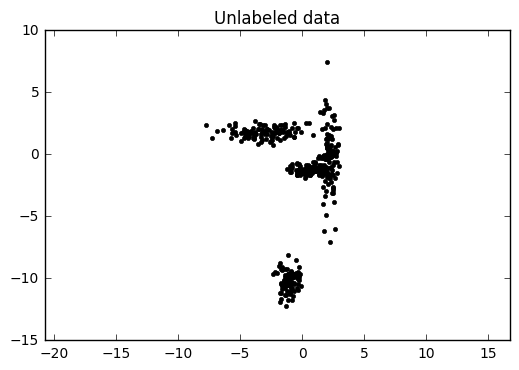
\includegraphics[height=5cm]{figures/unlabeled.png} &
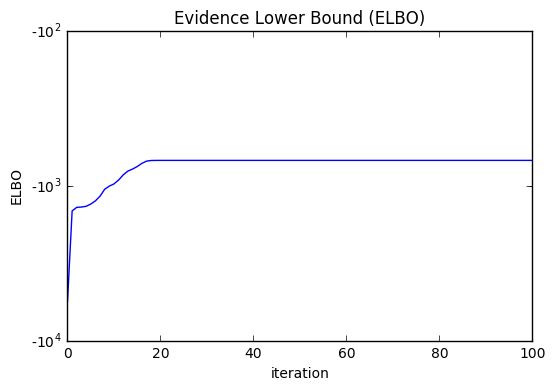
\includegraphics[height=5cm]{figures/elbo.png} \\
(a) & (b) \\[10pt]
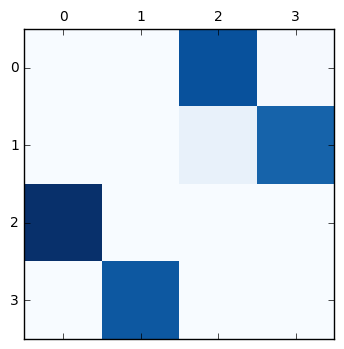
\includegraphics[height=5cm]{figures/confusion_matrix.png} &
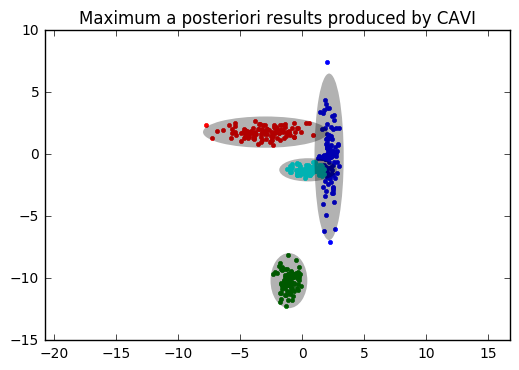
\includegraphics[height=5cm]{figures/cavi_max_a_posteriori.png} \\
(c) & (d)
\end{tabular}
\caption{Example results on a simulated dataset.
Plot (a) shows the unlabeled dataset,
(b) shows the ELBO evaluated during the course of training,
(c) shows the resulting confusion matrix computed relative to the true clustering,
and (d) shows the maximum a posteriori clustering results (the ellipses represent contours of the per-class Gaussians).}
\label{fig:resultsExample}
\end{figure}

\end{document}
